% Figure environments for the bandqr paper. Graphics live in ../figures/.
% Generated by figures.py; numbers quoted in captions are from benchmarks.ipynb.

\begin{figure}[t]
  \centering
  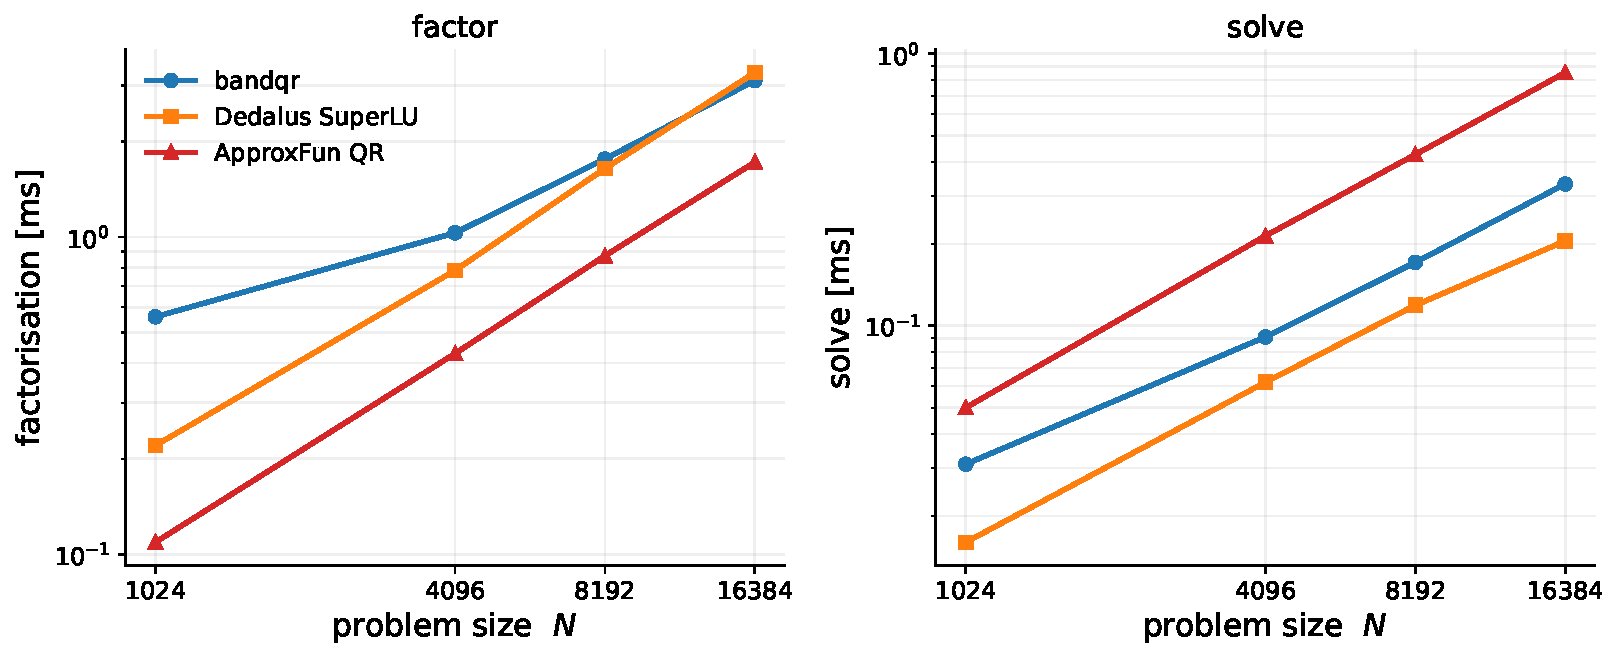
\includegraphics[width=0.85\textwidth]{figures/performance.pdf}
  \caption{Performance on the full almost-banded ultraspherical Helmholtz operator of
    size $N$ (banded bulk $+$ dense boundary-condition rows $+$ tau columns) --- all
    three methods solving the \emph{same} system, matrix assembly excluded,
    factorisation and solve timed separately (best of 15). \texttt{bandqr}'s ride-$\tau$
    method (ride for the dense rows, a Woodbury update for the tau columns) reproduces
    the direct solution to machine precision ($\sim\!10^{-15}$) and is \emph{competitive}
    with Dedalus's sparse-LU and \texttt{ApproxFun}'s almost-banded QR throughout, matching
    the sparse-LU factorisation and overtaking it modestly at large $N$ ($N\!\gtrsim\!12{,}000$,
    the crossover where bandqr's fixed set-up cost amortises). The point is not a large speed
    win---it is parity at machine precision with deterministic, pivot-free fill and
    unconditional backward stability; at small $N$ bandqr's fixed Python set-up still costs a
    little. The band-QR kernel itself is a small fraction of the total
    (Fig.~\ref{fig:bandwidth}).}
  \label{fig:performance}
\end{figure}

\begin{figure}[t]
  \centering
  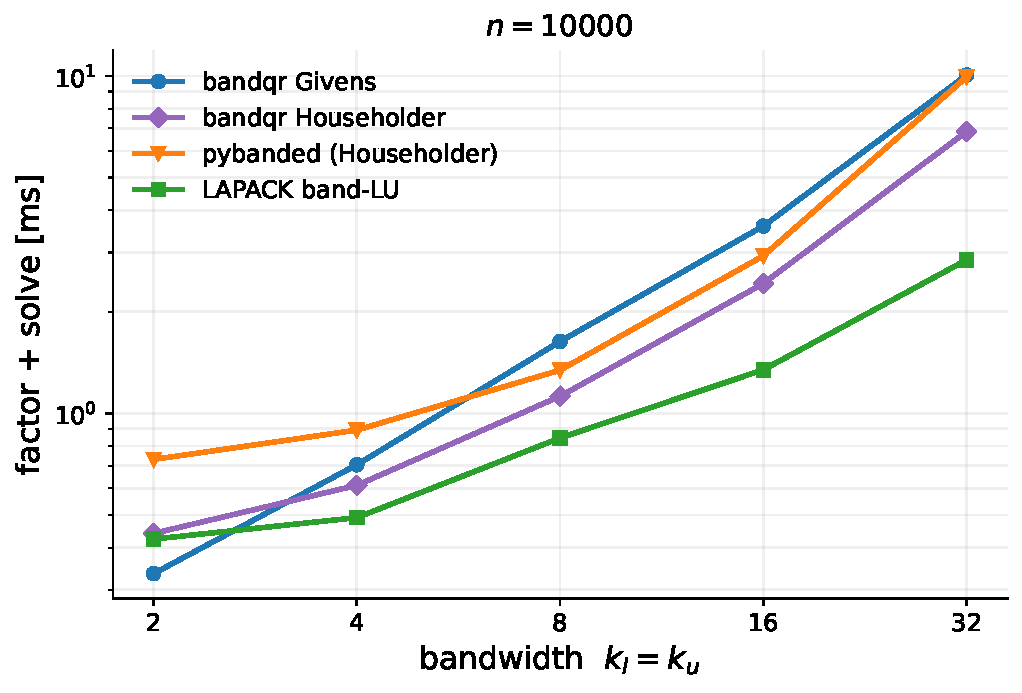
\includegraphics[width=0.62\textwidth]{figures/bandwidth.pdf}
  \caption{Factor-plus-solve time versus bandwidth $k_l=k_u$ for dense-banded
    systems of size $n=10000$ (best of~7), all methods on the same matrices.
    \texttt{bandqr}'s Givens variant is fastest at the narrowest bands typical of
    spectral discretisations ($k_l=2$), where it is also the fastest method overall;
    its Householder variant takes over among the QR methods at moderate-to-wide bands,
    beating the Dedalus-ecosystem banded QR \texttt{pybanded} (also Householder) by up
    to $\sim\!30\%$. LAPACK's blocked band-LU pulls ahead from $k_l\!\gtrsim\!4$, as
    expected---QR does strictly more work but, unlike pivoted LU, never densifies and
    has bandwidth-bounded, data-independent fill.}
  \label{fig:bandwidth}
\end{figure}

\begin{figure}[t]
  \centering
  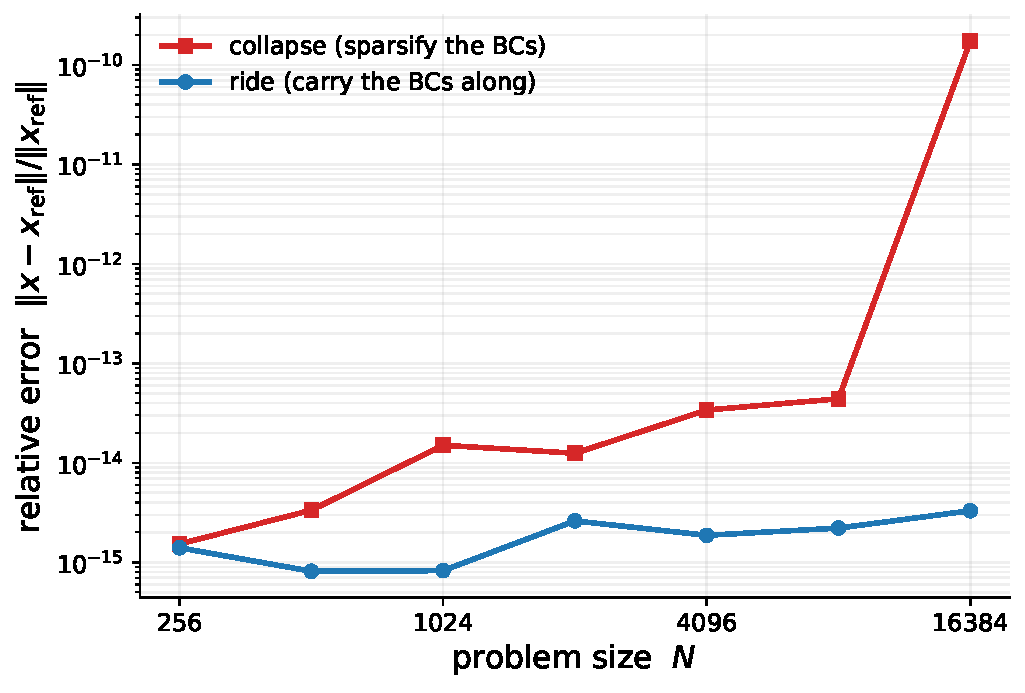
\includegraphics[width=0.62\textwidth]{figures/conditioning.pdf}
  \caption{Accuracy of the two boundary-row strategies on the Helmholtz operator,
    versus problem size $N$, measured as relative error against a sparse direct
    solve. \emph{Collapse} sparsifies the boundary rows into the band with the
    automatically detected recurrence; \emph{ride} carries them along as low-rank
    fill. Both are accurate at small $N$, but collapse conditions the preconditioned
    system and degrades to $\sim\!10^{-10}$ by $N=16384$, whereas ride stays at
    machine precision ($\sim\!10^{-15}$) throughout---five orders of magnitude
    better at the largest size. Collapse is simpler and keeps a single band; ride is
    the choice when robustness at large $N$ matters.}
  \label{fig:conditioning}
\end{figure}

\begin{figure}[t]
  \centering
  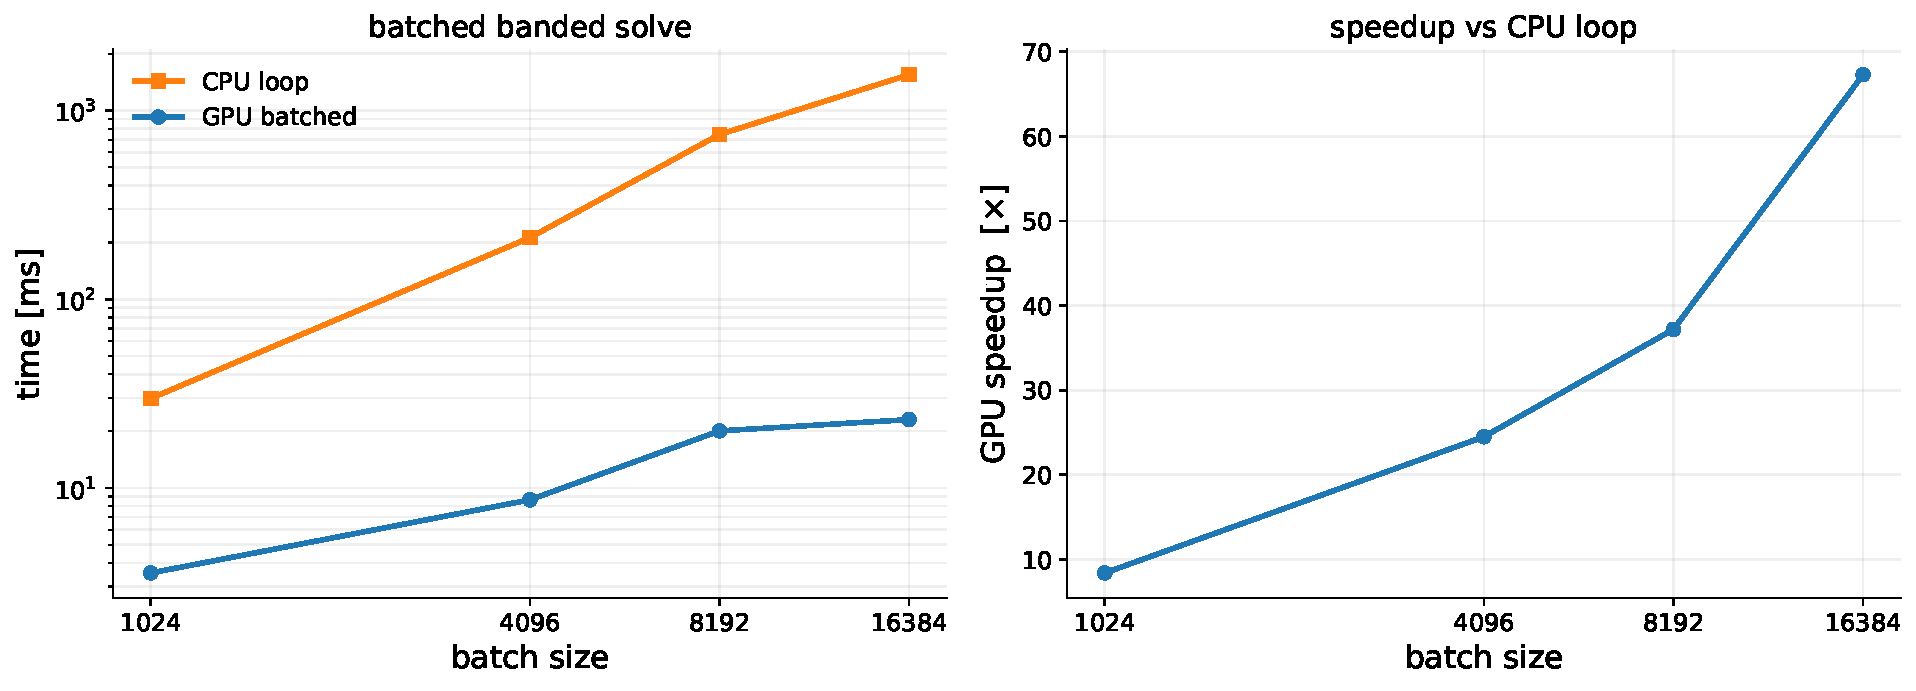
\includegraphics[width=\textwidth]{figures/gpu.pdf}
  \caption{Batched banded solve on the Apple GPU (\texttt{mlx}, single precision,
    one thread per system) against a CPU loop over the same systems, as the number
    of independent same-shape systems (the batch) grows. \emph{Left:} wall-clock
    time; \emph{right:} GPU speedup. Because the solver is pivot-free there is no
    warp divergence, and throughput scales with batch size, reaching $\sim\!67\times$
    at a batch of~16384. This is the regime of multidimensional spectral solves, where
    each transverse wavenumber yields an independent banded system.}
  \label{fig:gpu}
\end{figure}
